%%%
%%% setup.tex
%%%


\section{Modeling Constraints and Algorithm Overview}
\label{sec:setup}
%%%
%%% Introduction
%%%
In this section, we impose three constraints that the routing system
must satisfy to enable efficient and accurate route prediction.  

Next, we describe how these constraints enable us to decompose the
algorithm into three stages---applying the import policy to eBGP-learned
routes, selecting the best BGP route at each router, and computing the
forwarding path.  The algorithm takes as input the router configuration
and a static snapshot of the routes learned via eBGP and outputs the
route that each router in the AS selects, for each destination.  Because
the first and third stages of the algorithm are relatively simple, the
rest of the chapter focuses on the second stage of computing the best
BGP route at each router for each destination prefix.



\subsection{Modeling Constraints}
%%%
%%% Feasibility of such a model
%%%
Efficiently computing the effects of a configuration or topology change
is possible 
when three important conditions hold.  These constraints include the
various correctness properties specified in
Chapter~\ref{chap:rlogic} that can be verified with static configuration
analysis (Chapter~\ref{chap:rcc}).  Specifically, we assume that safety,
and the second condition of determinism are satisfied.  Imposing these
constraints free our prediction algorithms from needing to consider
whether different orderings of routing will produce different results.
This property allows us to focus on designing algorithms that emulate a
particular message ordering that prevents the algorithm from having to
revisit routers where it has already made a prediction.  The rest of
this section explains how these constraints and others help simplify the
prediction algorithms.

First, the inputs to the algorithm must be stable.  In particular,

\begin{constraint}[Slowly changing inputs]
\label{a:ebgp}
The eBGP-learned routes change slowly with respect to the timescale of
network engineering decisions.
\end{constraint}

\vspace*{0.1in}
\noindent
If the eBGP-learned routes change frequently, the internal routing
system does not have time to propagate the effects of one eBGP
advertisement before the next one arrives.  In practice, most BGP
routes are stable for days or weeks at a time~\cite{labovitz99}, and
the vast majority of traffic is associated with these stable
routes~\cite{Rexford:stability2002}.  This allows the routing algorithm to operate on
a static snapshot of the eBGP routes.  Any eBGP routing change can be
treated as a separate problem instance.

Second, the routers in the AS must ultimately reach a stable
outcome.  In particular,

\begin{constraint}[Safety and uniqueness]
\label{a:ibgp}
Given stable eBGP-learned routes and fixed iBGP and IGP topologies,
each router inside the AS converges to a unique routing decision.
\end{constraint}

\vspace*{0.1in}
\noindent
If the routers continually change the routes that they select,
accurately predicting how the flow of data traffic becomes significantly
more challenging.  Fortunately, previous work~\cite{Griffin2002} has
identified sufficient conditions for an internal routing configuration
to satisfy Constraint~\ref{a:ibgp}.  We describe these conditions in
more detail in Section~\ref{sec:best_egress} when we address the
challenges introduced by route reflectors.

Third, the routing decisions at each router should not depend on
message ordering or timing:

\begin{constraint}[Determinism, Condition \#2]
\label{a:determ}
The routing decision at each router depends only on the routes received
from its neighbors and {\em not} the order or timing of these routing
messages. 
\end{constraint}

\vspace*{0.1in}
\noindent
Some router vendors have an additional step in the BGP
decision process that favors the ``oldest'' route before the final
tie-breaking step of comparing the router IDs.  The ``age-based
tie-breaking'' favors more stable routes, making the outcome of the
BGP decision process dependent on the {\em order\/} the router
receives the advertisements (and, hence, violating determinism).
Disabling age-based tie-breaking forces 
a deterministic selection based on the smallest router ID, as in
Figure~\ref{tab:background:decision}; other BGP features, such as route flap
damping~\cite{rfc2439}, can help reduce the likelihood of selecting
unstable routes.


Constraint~\ref{a:ibgp}, which guarantees that the routing system will
converge to a unique outcome, and~\ref{a:determ}, which guarantees that
this outcome does not depend on the ordering of routing messages, allow
us to make the following observation:

\vspace{0.15in}
\begin{center}
\framebox{
\parbox{0.85\linewidth}{
\begin{observation}
\label{t:order}
If a routing system is guaranteed to converge to a unique outcome,
that outcome is independent of the order in which routers exchange routes
and apply the decision process.
\end{observation}
}
}
\end{center}
\vspace*{0.1in}
\noindent
This observation implies that the algorithm can consider the evolution
of the routing system under {\em any particular message ordering},
without the risk of arriving at the wrong answer.

%% note the properties that the algorithms do {\em not} require

It is worth noting that our algorithms do not require the routing system
to satisfy route validity or the first condition of determinism (recall
that determinism is only a sufficient condition for iBGP to satisfy
safety but is not necessary).  The algorithms in this chapter are only
concerned with predicting the outcome of BGP selection process, not
whether the resulting routes induce paths that violate route validity.  In
Sections~\ref{sec:med_model} and~\ref{sec:best_egress}, we permit
routers' selection functions to violate the first condition of
determinism because these violations capture BGP's default behavior
(\ie, this condition is violated whenever routers only compare the MED
attribute across routes received from the same neighboring AS).  The
algorithms do not explicitly require path visibility; rather, the
algorithms in
Sections~\ref{sec:simple} and~\ref{sec:med_model} implicitly assume path
visibility is satisfied (\ie, they assume a ``full mesh'' iBGP
configuration).

\subsection{Overview: Decomposing BGP Route Selection into Three
  Stages}\label{sec:decompose} 

\begin{figure*}
\centering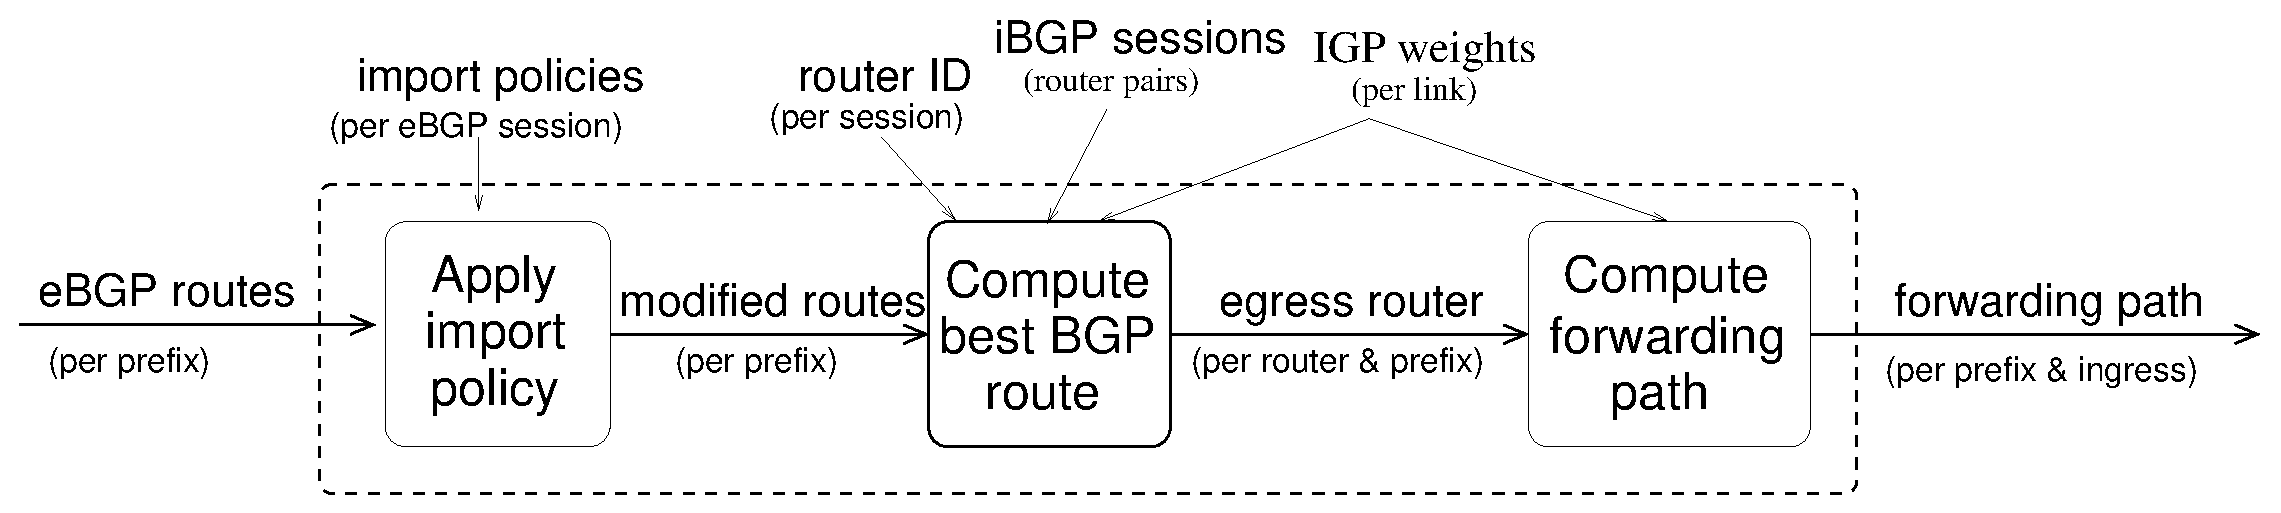
\epsfig{file=sandbox/figures/bigpic4.eps,width=\textwidth}
\caption[Decomposing BGP route selection into three
  independent stages.]{Our algorithms decompose network-wide BGP route
  selection into three independent stages.  The algorithms take as input
  the eBGP-learned routes from neighboring ASes, the router IDs of each
  BGP session, and the routing configurations from all of the routers in
  the AS, which provide information about the IGP topology, the iBGP
  topology, and the import policies (\ie, rankings) of each router.}
\label{fig:modules}
\end{figure*}

Following the approach applied in other recent
work~\cite{Feamster2005b,Gao2001a}, the algorithms in this chapter
compute the effects of a particular message ordering using an {\em
activation sequence\/}, an {\em offline} analysis technique that
``activates'' one or more routers at each discrete step.  When
activated, a router applies the decision process in
Table~\ref{tab:background:decision} and propagates the best route to its
iBGP neighbors.  Our algorithms are based on an activation sequence that
allows us to decompose route prediction into three distinct stages, as
shown in Figure~\ref{fig:modules}:

\textbf{1. Receiving the eBGP routes and applying import policy.} This
stage takes as input all of the eBGP-learned routes at each router and
applies the appropriate import policies at each router {\em before
exchanging any iBGP update messages} and outputs the set of eBGP-learned
routes after these import policies have been applied.  This stage
activates all of the edge routers at the same time.  

Each eBGP-learned route has attributes (such as the destination prefix
and the AS path) and is associated with an eBGP session.  The import
policy may filter the route or set certain attributes such as local
preference, origin type, and multiple-exit discriminator (MED),
according to attributes in the advertised route (\eg, based on ASes in
the AS path).  Because applying the import policy is a local operation
for each eBGP-learned route at each router, the first stage emulates the
operations a real router would perform upon receiving each of the eBGP
routes.  These routes, with modified attributes, are the input to the
second stage.

\textbf{2. Computing the best BGP route at each router.}  When iBGP
satisfies path visibility, many routes from the first stage could never
be selected by any router as the best route.  For example, an
eBGP-learned route with a local preference of 90 would {\em never} be
selected over another route with a local preference of 100.  In
addition, different routers in the AS may select different best BGP
routes because they have different IGP path costs to the egress router.
Also, a router can only consider the routes advertised by its iBGP and
eBGP neighbors, which may influence the final decision at that router.
%Deriving accurate and
%efficient algorithms for computing the best BGP route at each router
%is the main contribution of this paper.  
This stage takes as input the set of eBGP-learned routes after the
import policies of each router have been applied and outputs a single
best egress router for each ingress router and destination prefix.
Constructing an efficient activation sequence for this stage is
challenging, and is the focus of the next four sections of the chapter.

Using Observation~\ref{t:order}, our goal is to devise an {\em
activation sequence\/}, which ``activates'' one or more routers at any
given phase.  When activated, a router $r$ applies the BGP decision
process to compute a best route from its available candidate routes,
which it then may propagate to other routers via iBGP.  In an actual
network, routers may be activated in any order and may change their best
route many times before the network converges.  This chapter focuses on
devising activation sequences that allow us to efficiently compute
the final routing decision.


\textbf{3. Computing the forwarding path through the AS:} The third
stage of the algorithms compute the effects of the IGP link weights on
the construction of the forwarding path through the AS from an ingress
router toward a destination prefix.  Given the selected BGP route, the
ingress router forwards packets along the outgoing link (or links) along
shortest paths to the egress router, and the process repeats at the next
router.  Ideally, the traffic flows along the shortest path (or paths)
all the way from the ingress router to the selected egress router.
However, in practice, routers along the shortest path may have selected a
{\em different} egress router, thus violating route validity
(Definition~\ref{defn:rv}).  These 
violations can occur if the iBGP session configuration limits the
BGP routing options at the routers~\cite{Griffin2002}.  By considering
one router at a time, the third stage can compute an accurate view of
the forwarding path(s) even when deflections occur.

While all three steps are necessary for determining the flow of traffic
through a network from a static snapshot of the network state, the rest
of this chapter focuses on the second step (\ie, computing the best BGP
route at each router), since performing this step correctly and
efficiently is considerably more difficult than either of the other two
steps.
